\section{Introduction}
\label{sec:introduction}

Graphics processing units (GPUs) are becoming powerful many-core compute
devices.
For example, NVIDIA GPUs integrate more than $1,500$ processing cores on
a single chip and the peak double-precision performance exceeds 1
TFLOPS while sustaining thermal design power (TDP) in the same order of
magnitude as traditional multicore CPUs~\cite{NVIDIA_Kepler}. 
This rapid growth of GPUs is due to recent advances in the
programming model, often referred to as general-purpose computing on
GPUs (GPGPU).
Current main applications of GPGPU can be found
in supercomputing~\cite{TOP500} but there are more and more emerging
applications in many different fields.
Examples include plasma control~\cite{Kato_ICCPS13}, autonomous
driving~\cite{McNaughton_ICRA11}, software routing~\cite{Han_SIGCOMM10},
encrypted networking~\cite{Jang_NSDI11}, and storage
management~\cite{Bhatotia_FAST12, Gharaibeh_HPDC10, Kato_ATC12,
Sun_SYSTOR12}.
This broad range of applications raises the need of understanding
the systematic behavior of GPU computing.

\begin{figure}[!t]
 \centering
 \subfigure[Host to Device]{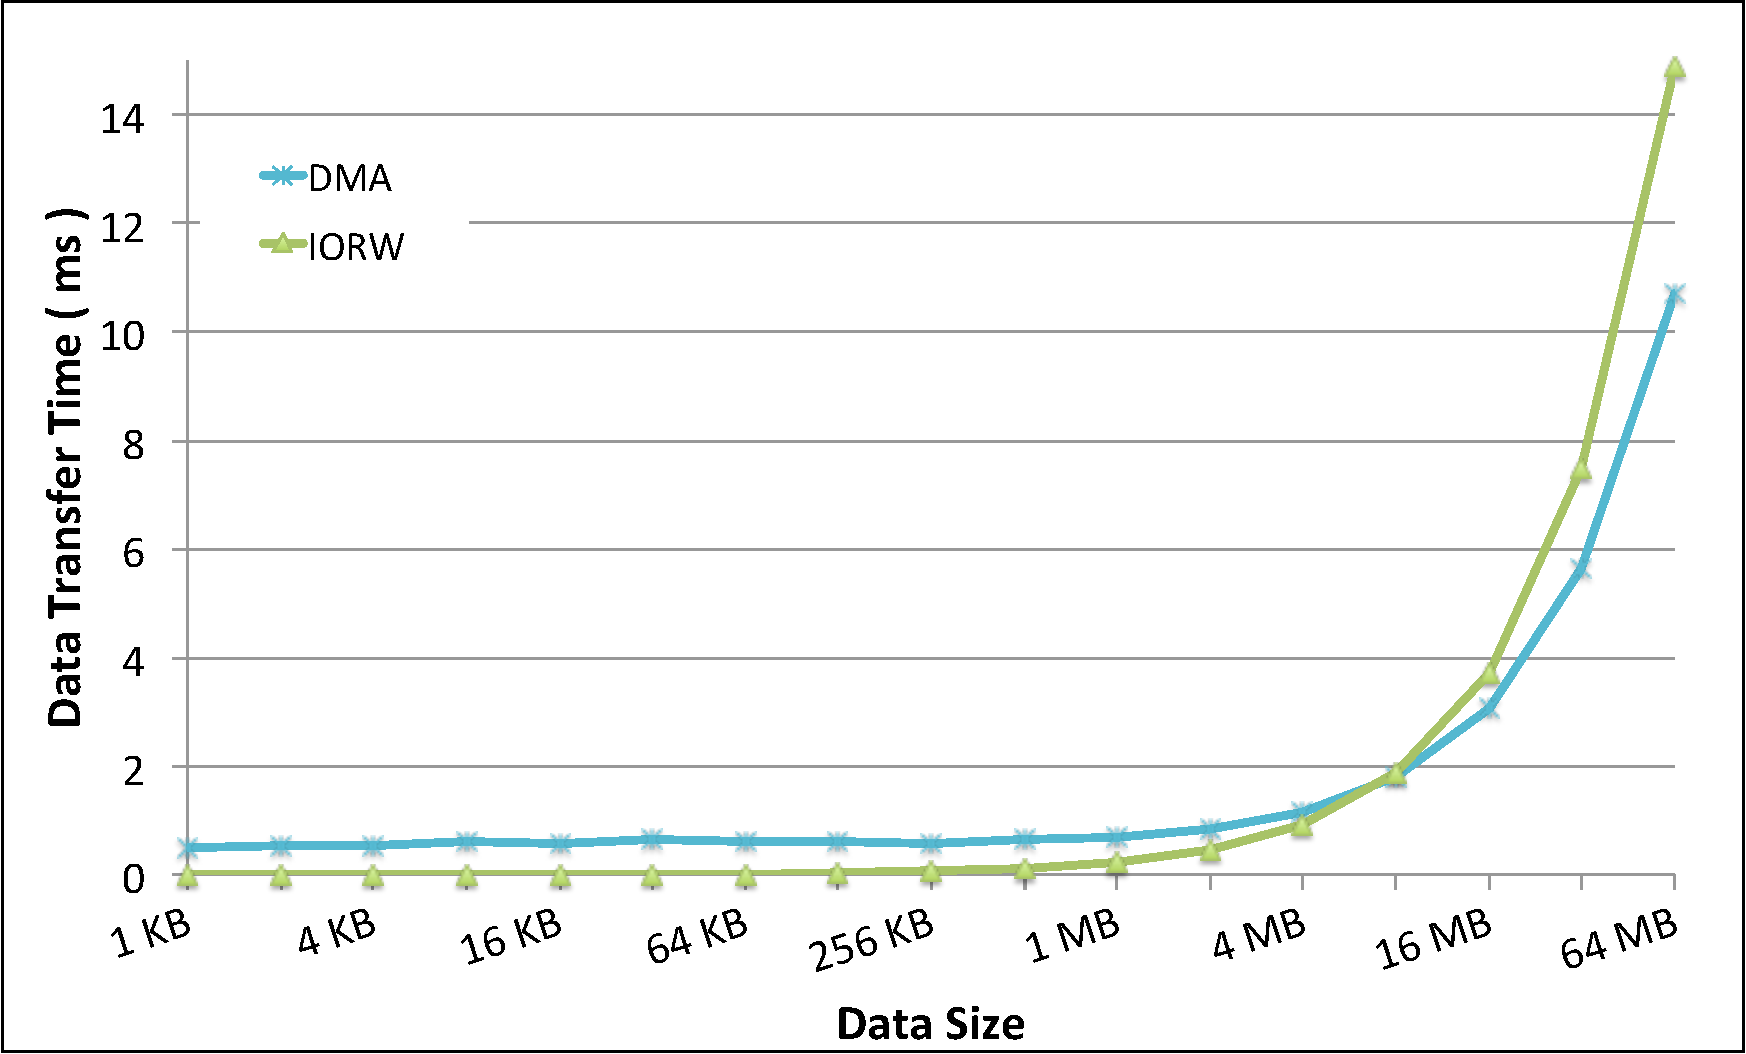
\includegraphics[width=0.34\textwidth]{figure/Graph/forIntro_HtoD.pdf}}\\
 \subfigure[Device to Host]{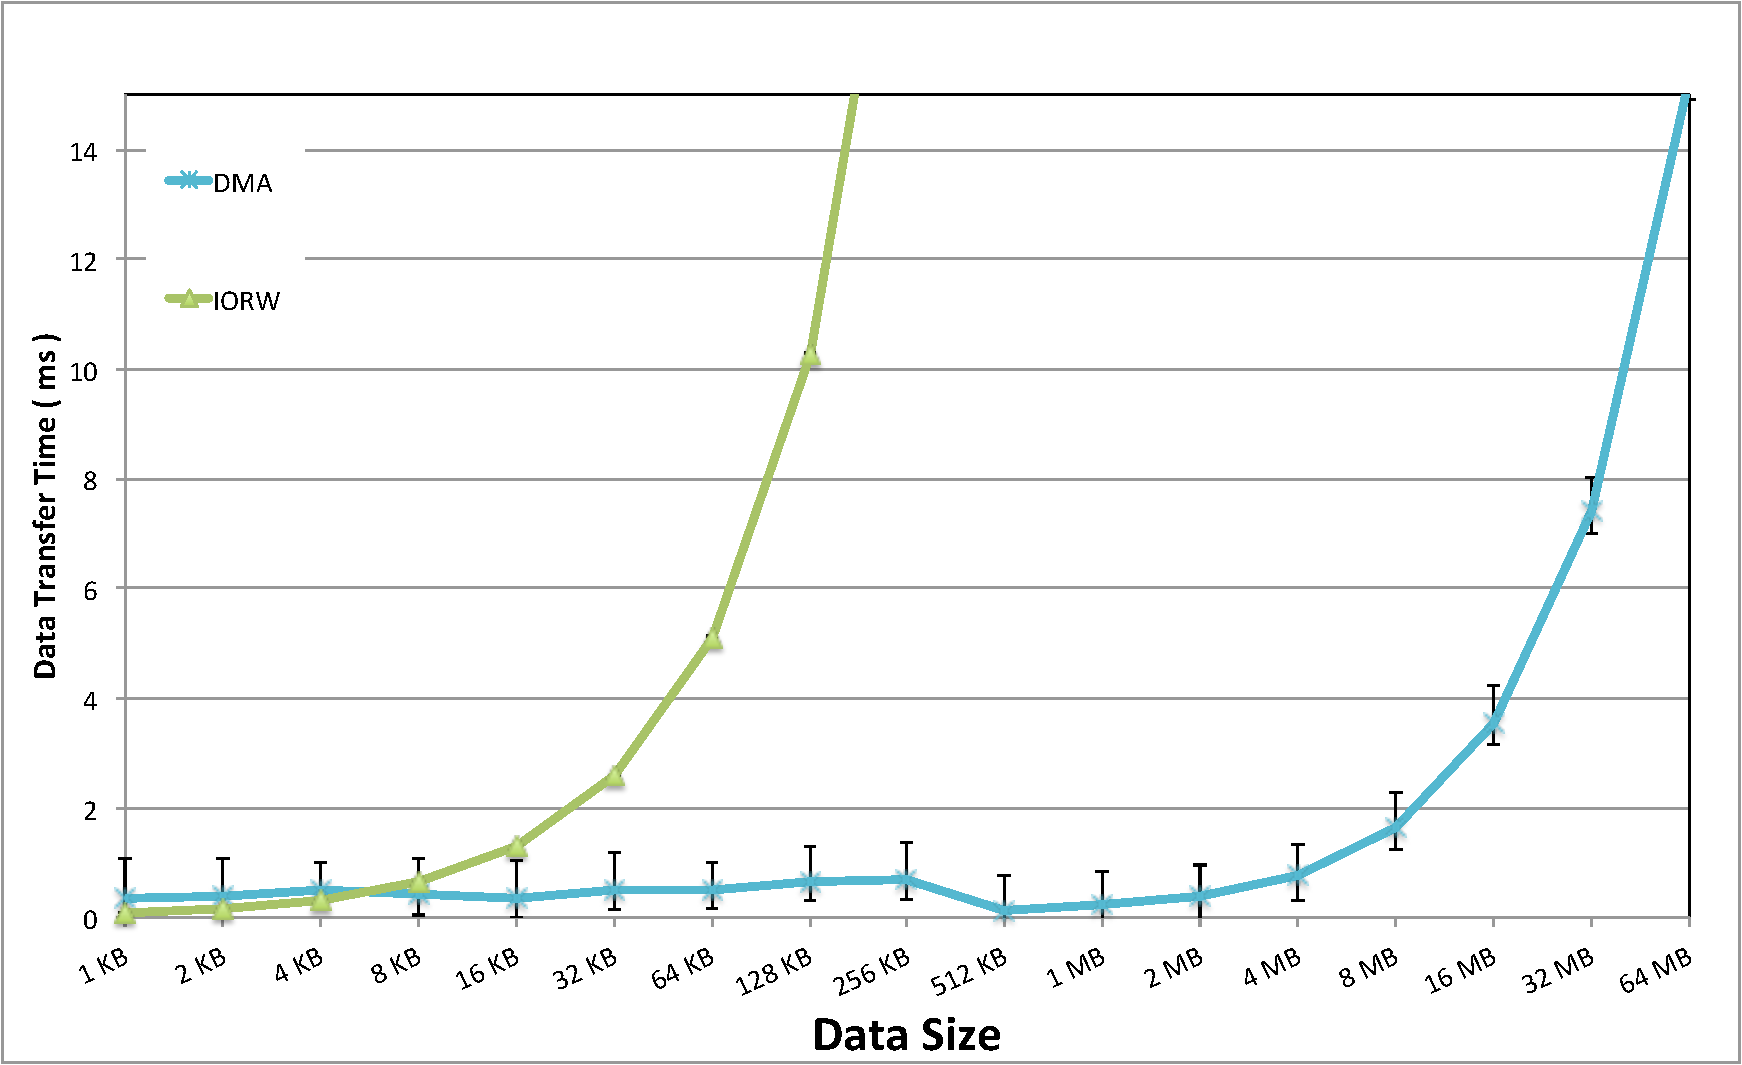
\includegraphics[width=0.34\textwidth]{figure/Graph/forIntro_DtoH.pdf}}
 \caption{Performance of DMA and I/O read/write for the GPU.}
 \label{fig:intro_data_transfer}
\end{figure}

GPU computing in the current state of the art contains many black-box
pieces, though open-source contributions of system software started
appearing~\cite{Kato_ATC11, Kato_ATC12}.
Current systems hence rely on closed-source propriately software
provided by the vendors, praying that the black-box pieces are well
designed to optimize performance.

prevent from understanding 

One of the greatest challenges of GPU computing is the management of
latency issues.

nobody knows